\begin{multicols}{3}
\bylineDE{Interview mit Frau Brigitte Weißörtel}{Silviya  XI D}

  \noindent 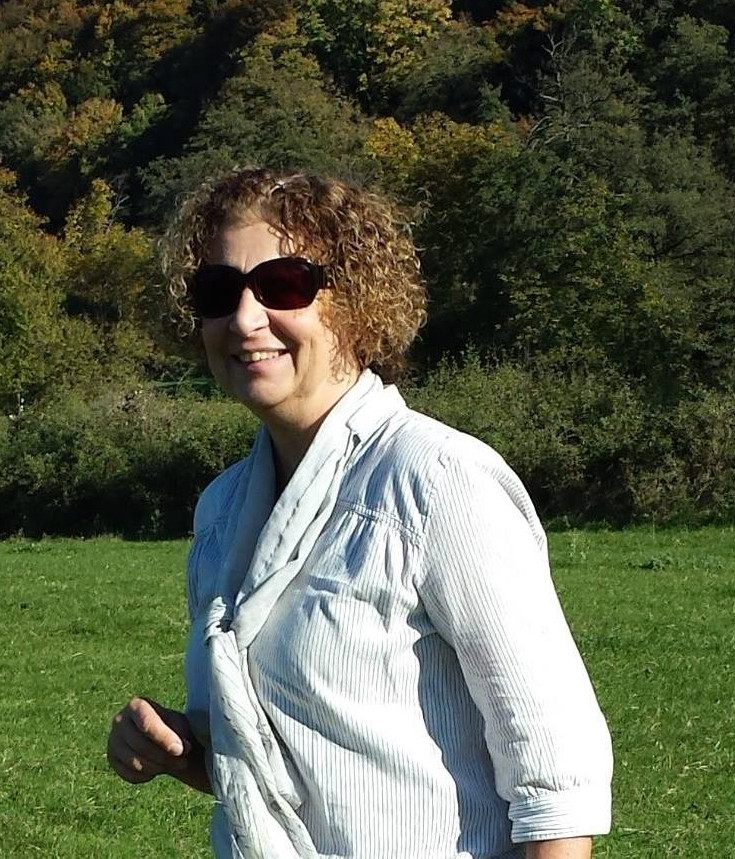
\includegraphics[width=2.1in]{./Brigitte/6.jpg}

Wie kamen Sie ans Goethe-Gymnasium nach Burgas?

Ich habe mich weltweit  für den Auslandschuldienst beworben und , bin davon ausgegangen, dass ich an eine Deutsche Schule geschickt werde und dort Geographie und Englisch unterrichte. 
Aber dann kam von der Zentralstelle für das Auslandsschulwesen in Köln ein sehr verlockendes Angebot: die Stelle einer Fachschaftsberaterin in Bulgarien. Und so unterrichte ich jetzt Deutsch als Fremdsprache, bin für die Abwicklung des DSD in Burgas und Ruse zuständig, halte Fortbildungsveranstaltungen für bulgarische Deutschlehrkräfte und konnte hier an meiner Stammschule einen neuen Deutschraum mit Lesebücherei einrichten. Und diese Vielfalt bei der Arbeit gefällt mir ausgesprochen gut. 

Erfüllen die bulgarischen Schüler  Ihre Erwartungen?

Es sind schon große Kulturunterschiede zu Deutschland festzustellen. Das Unterrichten hier bereitet mir große Freude, besonders deswegen, weil die bulgarischen Schüler Unterrichtsmethoden, die ihnen völlig neu sind, gerne und dankbar annehmen. Und von ihrem hohen Sprachniveau bin ich sehr beeindruckt. 

Können wir das Verhalten der bulgarischen mit dem der deutschen Schüler vergleichen?

Bulgarische Schüler lernen viel auswendig und diskutieren wenig. Deutsche Schüler sagen offen ihre Meinung, bei den bulgarischen bin ich oft nicht sicher, ob das wirklich ihre Meinung ist, was sie sagen.
Dass Schüler wochenlang nicht im Unterricht sind, weil sie anderen Aktivitäten nachgehen... das gibt es in Deutschland nicht. 

Sind  die gute Vorbereitung und das niedrige Selbstbewusstsein besser für die DSD-Prüfung oder die nicht so gute Vorbereitung , aber mit hohem Selbstbewusstsein?

Das hängt eng zusammen. Wenn man gut vorbereitet ist, kommt man selbstbewusst in die Prüfung (und umgekehrt)

Der beste Charakterzug der Deuschen ist… ?

Die Zuverlässigkeit.

Wie beschreiben Sie die Bulgaren?

Vielen Bulgaren, die ich kennengelernt habe, würde ich etwas mehr Selbstbewusstsein wünschen 

Personen die Sie inspirieren?

Nelson Mandela, Dr Martin Luther King und Willi Brandt.

Glauben Sie, dass eine Frau in der Politik die Welt viel besser machen kann?

Jedenfalls wird sie nicht schlechter als ein Mann arbeiten.

Planen Sie Bulgarien noch ein Mal zu besuchen?

Ich bleibe ja noch einige Zeit hier; danach komme ich vielleicht mal im Urlaub her(aber nicht an den Sonnenstrand!)
 \closearticle
\end{multicols}